\section{Renyi divergenca glede na histogram}\label{posplositev1d}

Zdaj, ko dobro poznamo pojem histograma, lahko definiramo Renyi divergenco glede na histogram. Histogram bo torej ocena za gostoto verjetnosti vzorca.

V prejšnjem poglavju smo omenili, da lahko histogram predstavimo kot funkcijo, a bo za računanje Renyi divergence boljše, da si histogram predstavljamo grafično. Torej predstavljamo si ga kot skupek pravokotnikov (stolpcev) z določenimi mejami in višinami.

\subsection{Formula za računanje Renyi divergence glede na histogram}

\begin{izrek}
    Naj bo $H_1$ histogram, ki ima meje stolpcev $(x_0,x_1,\ldots,x_{n-1}, x_n)$ in višine stolpcev $(h_{(1,0)},\ldots,h_{(1,n-1)})$. Naj bo $H_2$ histogram, ki ima meje stolpcev iste kot $H_1$ in višine stolpcev $(h_{(2,0)}, \ldots, h_{(2,n-1)})$ (torej imata $H_1$ in $H_2$ isto število stolpcev in enake meje, le različne višine). Tedaj lahko Renyi divergenco med histogramoma $H_1$ in $H_2$ izračunamo kot:
    \begin{equation}
        D_\alpha (H_1 \| H_2) = \frac{1}{\alpha-1} \log\Big(\sum_{i=0}^{n-1} h_{(1,i)}^\alpha \cdot h_{(2,i)}^{1-\alpha} \cdot (x_{i+1}-x_i)\Big),
    \end{equation}
    če $\alpha \neq 1$, oziroma
    \begin{equation}
        D_1 (H_1 \| H_2) = \sum_{i=0}^{n-1} h_{(1,i)}\cdot \log \frac{h_{(1,i)}}{h_{(2,i)}} \cdot (x_{i+1}-x_i).
    \end{equation}
\end{izrek}

\begin{proof}
    Vemo: če $H_1$ in $H_2$ zapišemo kot funkciji ($H_1 = H_1 (x)$ in $H_2 = H_2(x)$), dobljeni funkciji ustrezata pogojem za gostoto verjetnosti. Torej lahko izračunamo Renyi divergenco po definiciji:
    \begin{equation}
        D_{\alpha} (H_1 \| H_2) = \frac{1}{\alpha-1} \log\int_{x_0}^{x_n} H_1(x)^\alpha \cdot H_2(x)^{1-\alpha} dx.
    \end{equation}
    Ker sta funkciji $H_1$ in $H_2$ nezvezni v istih točkah (v mejah stolpcev), zapišemo integral kot vsoto integralov na intervalih, kjer sta $H_1$ in $H_2$ konstantni:
    \begin{equation}
        \int_{x_0}^{x_n} H_1(x)^\alpha \cdot H_2(x)^{1-\alpha} dx = \int_{x_0}^{x_1} H_1(x)^\alpha \cdot H_2(x)^{1-\alpha} dx + \ldots + \int_{x_{n-1}}^{x_n} H_1(x)^\alpha \cdot H_2(x)^{1-\alpha} dx.
    \end{equation}
    Če upoštevamo še konstantne vrednosti funkcij $H_1$ in $H_2$ na intervalih integriranja, in v vsakem členu integriramo $\int_a^b dx = b-a$, dobimo:
    \begin{equation}
        h_{(1,0)}^\alpha\cdot h_{(2,0)}^{1-\alpha}\cdot (x_1-x_0) + \ldots + h_{(1,n-1)}^\alpha\cdot h_{(2,n-1)}^{1-\alpha}\cdot (x_n-x_{n-1}) = \sum_{i=0}^{n-1} h_{(1,i)}^\alpha \cdot h_{(2,i)}^{1-\alpha} \cdot (x_{i+1}-x_i),
    \end{equation}
    torej je:
    \begin{equation}
        D_\alpha (H_1 \| H_2) = \frac{1}{\alpha-1} \log\Big(\sum_{i=0}^{n-1} h_{(1,i)}^\alpha \cdot h_{(2,i)}^{1-\alpha} \cdot (x_{i+1}-x_i)\Big).
    \end{equation}
    Podobno dokažemo za $\alpha = 1$ - izračunamo Kullback-Leibler divergenco.
\end{proof}

Zdaj znamo izračunati Renyi divergenco med dvema histogramoma, a imamo zelo strogo omejitev: meje stolpcev prvega histograma morajo biti enake mejam stolpcev drugega histograma. Opišimo, kako v splošnem primeru zadostimo tej omejitvi, brez da spreminjamo ploščine histogramov.

% rezanje histogramov
\subsection{Sprostitev definicijskega območja histogramov} \label{podpoglavje-4-1}

Če hočemo, da imata poljubna histograma enake meje stolpcev, moramo najprej uskladiti definicijski območji histogramov.

Naj bo $X$ urejen seznam z mejami stolpcev prvega histograma in $Y$ urejen seznam z mejami stolpcev drugega histograma. Za spodnjo mejo:
\begin{itemize}
	\item Če je $\min(X) > \min(Y)$, potem na začetek seznama $X$ vstavimo element $\min(Y)$. Tako v prvem histogramu dobimo še en stolpec z mejami $\min(Y)$ in $\min(X)$. Dodelimo mu vrednost $0$.
	\item Če je $\min(X) < \min(Y)$, potem na začetek seznama $Y$ vstavimo element $\min(X)$. Tako v drugemu histogramu dobimo še en stolpec z mejami $\min(Y)$ in $\min(X)$. Dodelimo mu vrednost $0$.
\end{itemize}
Za zgornjo mejo:
\begin{itemize}
	\item Če je $\max(X) < \max(Y)$, potem na konec seznama $X$ vstavimo element $\max(Y)$. Tako v prvem histogramu dobimo še en stolpec z mejami $\max(X)$ in $\max(Y)$. Dodelimo mu vrednost $0$.
	\item Če je $\max(X) > \max(Y)$, potem na konec seznama $Y$ vstavimo element $\max(X)$. Tako v drugem histogramu dobimo še en stolpec z mejami $\max(Y)$ in $\max(X)$. Dodelimo mu vrednost $0$.
\end{itemize}
Dobili smo torej največ dva nova stolpca. Ker smo jima dodelili vrednost $0$, ploščina histograma ostaja enaka, torej je bil to dober korak k našemu cilju (da bodo ploščine histogramov čim bližje 1). Definicijsko območje obeh histogramov je na sedaj enako.

\begin{zgled}

Poglejmo si primer, kako sprostimo definicijsko območje histograma.

\begin{figure}[!bh]
    \centering
    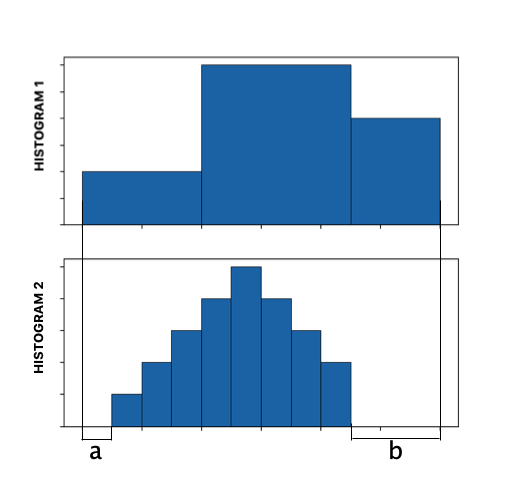
\includegraphics[scale=0.7]{definicijskoobmocje}
    \caption{Sprostitev definicijskega območjahistograma 2. Dobili smo dva nova stolpca ain b.}
\end{figure}

\end{zgled}
\pagebreak
\subsection{Prerazporeditev mej v histogramih}
Ko imamo histograma, definirana na enakem definicijskem območju, moramo uskladiti še meje stolpcev obeh histogramov. To naredimo tako, da združimo meje prvega in drugega histograma.

Naj bo $X$ urejen seznam z mejami prvega histograma in $Y$ urejen seznam z mejami drugega histograma. Tvorimo seznam $Z = X \cup Y$ in ga uredimo po velikosti od najmanjšega do največjega. Dolžina seznama $Z$ naj bo enaka $n$. Cilj je, da imata na koncu naša histograma razporeditev stolpcev ravno $Z$. Zdaj že vemo, da imata $X$ in $Y$ enak prvi in zadnji element (zaradi sprostitve definicijskega območja). Naj predstavlja zapis $A(i)$ i-ti element seznama $A$, vsak seznam pa vedno začnemo šteti z 1.

Ker že vemo, da bo na koncu veljala enakost $X = Z$, se osredotočimo le na vrednosti oz. višin stolpcev v prvem histogramu z novimi mejami.

Brez škode za splošnost lahko rečemo,  da je vrednost stolpca dodeljena prvi (manjši) meji stolpca. Tako ima vsak element $X(i)$ dodeljeno vrednost $X_v(i)$, ki predstavlja višino stolpca z mejami $X(i)$ in $X(i+1)$. Zadnji meji ni dodeljena nobena vrednost, brez škode za splošnost mu lahko priredimo vrednost 0.

Z zanko se sprehodimo čez seznam $Z$ (t.j. $i = 1, \cdots, n-1$, kjer je $n$ enak dolžini seznama $Z$) in ga primerjajmo s seznamom $X$. Vsakemu elementu $Z$ želimo dodeliti vrednost, tako da bo histogram z mejami $Z$ sovpadal s histogramom z mejami $X$. Prva elementa sta enaka, zato elementu $Z(1)$ dodelimo vrednost $X_v(1)$. Za vsak naslednji $i$ imamo dve možnosti:
\begin{itemize}
	\item Če je $Z(i) = X(i)$, elementu $Z(i)$ priredimo vrednost $X_v(i)$. 
	\item Če je $Z(i) \neq X(i)$, potem elementu $Z(i)$ priredimo enako vrednost, kot jo priredimo meji $Z(i-1)$, torej vrednost $X_v(i-1)$.
\end{itemize}
Za prvi histogram torej dobimo meje stolpcev $Z$ in višine stolpcev $Z_{v1}$, kjer je za $i = 1, \cdots, n-1$ elementu $Z(i)$ prirejena vrednost $Z_{v1}(i)$, zadnjemu elementu v seznamu $Z$ pa priredimo vrednost $0$.

Analogno primerjamo seznam $Z$ in $Y$. Tako za drugi histogram dobimo meje stolpcev $Z$ in višine stolpcev $Z_{v2}$, kjer je za $j = 1, \cdots, n-1$ elementu $Z(j)$ prirejena vrednost $Z_{v2}(j)$, zadnjemu elementu v seznamu $Z$ pa priredimo vrednost $0$.

Z zgornjim postopkom smo stolpce le "razbili" na več stolpcev z isto višino, tako da ploščina histograma ostaja enaka $1$.

\begin{zgled}
Na primeru iz podpoglavja \ref{podpoglavje-4-1} si poglejmo rezanje stolpcev.
\begin{figure}[h!]
	\centering
	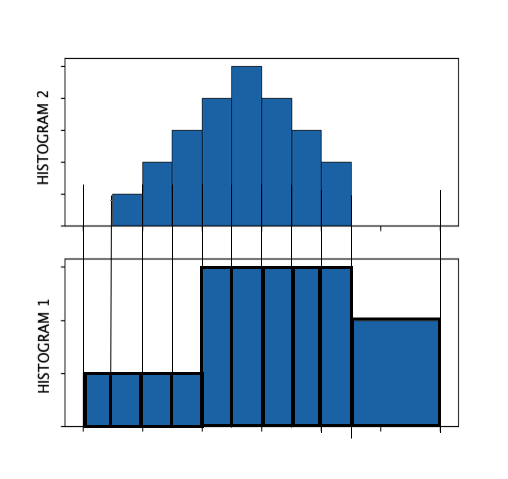
\includegraphics[scale=0.7]{prerazporeditev}
	\caption{Prerazporeditev mej stolpcev histograma 1 glede na histogram 2.}
    \end{figure}
    
\end{zgled}

Do sedaj smo med seboj primerjali le dve porazdelitvi. V nadaljevanju nas bo zanimal način, s katerim lahko primerjamo več porazdelitev hkrati. Za to pa moramo najprej vpeljati pojem entropije.